\newpage

\section{Вычислительный эксперимент}

Для анализа предложенного метода проводится вычислительный эксперимент для задачи прогнозирования временного ряда на $K=5$ шагов. 

В качестве тестируемых моделей используются архитектуры Кодировщика - Декодировщика~\cite{EncoderDecoder} на основе рекуррентной сети LSTM~\cite{LSTM1, LSTM2} и модели трансформера~\cite{Attention is all you need}.

Эксперимент проводится для выборок с размером входного окна, равного 5, 15 и 30. Каждая из выборок состоит из обучающей и тестовой части.


\begin{table}[H]
\begin{center}
\caption{Выборки}
\label{datasets}
\resizebox{\linewidth}{!}{
\begin{tabular}{|c|c|c|c|}
\hline
	Выборка & Пояснение & Размер входного окна & Горизонт прогнозирования \\
	\hline
	\multicolumn{1}{|l|}{YNDX-Train5}
	& Обучающая часть & 5 & 5 \\
	\hline
	\multicolumn{1}{|l|}{YNDX-Test5}
	& Тестовая часть & 5 & 5 \\
	\hline
	\multicolumn{1}{|l|}{YNDX-Train15}
	& Обучающая часть & 15 & 5 \\
	\hline
	\multicolumn{1}{|l|}{YNDX-Test15}
	& Тестовая часть & 15 & 5 \\
	\hline
	\multicolumn{1}{|l|}{YNDX-Train30}
	& Обучающая часть & 30 & 5 \\
	\hline
	\multicolumn{1}{|l|}{YNDX-Test30}
	& Тестовая часть & 30 & 5 \\
\hline
\end{tabular}
}
\end{center}
\end{table}

Для решения оптимизационной задачи используется градиентный метод оптимизации Adam~\cite{Adam}.

Для анализа качества моделей используются метрики: \\
1) Средняя квадратичная ошибка \\
2) Корреляция Пирсона, усредненная по каждому шагу прогнозирования (далее - Корреляция Пирсона)

\newpage

\subsection{ARIMA}

В качестве базовой модели прогнозирования используется архитектура ARIMA~\cite{ARIMA} с порядком дифференцирования $d = 0$, поскольку передаваемый ряд приведен к стационарному виду.

$$ ARIMA(p, d=0, q): $$
$$ y_{t} = \alpha_{1} y_{t-1} + ... + \alpha_{p} y_{t-p} + \varepsilon_{t} + \beta_{1} \varepsilon_{t-1} + \beta_{2} \varepsilon_{t-2} + ... + \beta_{q} \varepsilon_{t-q}, $$
где \\
$y_{t}$ - стационарный временной ряд, \\
$\alpha_{1}, ..., \alpha_{p}, \beta_{1}, ..., \beta_{q}$ - константы ($\alpha_{p} \neq 0, \beta_{q} \neq 0$), \\
$ \varepsilon_{t}$ - гауссов белый шум с нулевым средним и постоянной дисперсией.

Модели-кандидаты обучаются на первых 80 \% данных. Итоговый порядок модели определятся с помощью информационного критерия Акаике:
$$ AIC = -2\log{\mathcal{L}} + 2k,$$
где \\
$\mathcal{L}$ - значение функции правдоподобия модели, \\
$k = p + q + 1$ - количество параметров модели 

Качество полученной модели $ARIMA(p=3, d= 0, q=3)$ оценивается на оставшихся 20 \% данных для задачи прогнозирования на K шагов.

\begin{table}[H]
\begin{center}
\caption{Качество моделей}
\label{arima_quality}
\resizebox{\linewidth}{!}{
\begin{tabular}{|c|c|c|c|c|}
\hline
\textbf{Выборка} & \textbf{Модель} & \textbf{\begin{tabular}[c]{@{}c@{}}Дополнительные\\ данные\end{tabular}} & \textbf{\begin{tabular}[c]{@{}c@{}}Корреляция\\ Пирсона\end{tabular}} & \textbf{MSE} \\
\hline
\hline
& ARIMA & & $0{,}340$ & $0{,}0183$ \\
\hline
\end{tabular}
}
\end{center}
\end{table}

В таблице~\ref{arima_quality} представлены результаты сравнения полученных моделей.

\newpage 

\begin{figure}[H]\center
{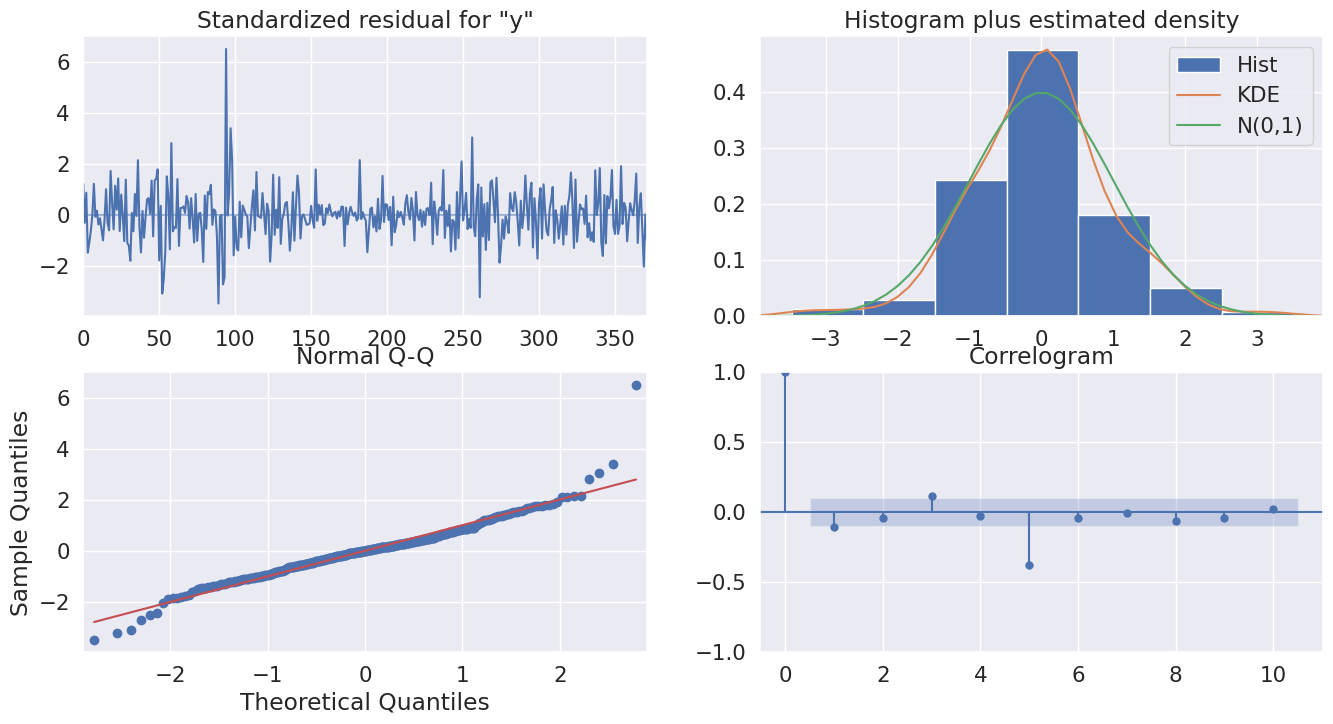
\includegraphics[width=1.0\textwidth]{results/residuals.png}}
\caption{Остатки ARIMA}
\label{residuals}
\end{figure}

Остатки модели - разница между фактическими значениями и значениями, прогнозируемыми моделью. \\

На рис.~\ref{residuals} показана диагностика полученной модели: \\
1) График остатков позволяет увидеть, равномерно ли распределены остатки вокруг нуля \\ 
2) Гистограмма остатков помогает визуально оценить, нормально ли распределены остатки \\
3) Q-Q plot сравнивает распределение остатков с нормальным распределением\\
4) График автокорреляционной функции остатков показывает автокорреляцию остатков на разных лагах \\

Исходя из полученных графиков следует вывод, что остатки модели не содержат дополнительной информации, важной для улучшения качества модели.

\newpage
\subsection{Модель автоследования} 

В качестве предложенного метода повышения качества моделей прогнозирования временных рядов предлагается использовать агрегированные знания опытных инвесторов.

Автоследование --- способ инвестирования, при котором все желающие могут подключиться к стратегии более опытного инвестора (он же автор стратегии) и автоматически повторять все его сделки на своем счете. 

Для создания модели автоследования выделяются инвесторы - авторы стратегий автоследования Тинькофф инвестиций. 
\[\text{Ответ инвестора} = \frac{\text{Сумма сделки}}{\text{Объем портфеля}}\]

При этом не рассматриваются сделки, сумма которых превышает объем портфеля.
 Путем усреднения ответов инвесторов о продаже или покупке акций составляется временной ряд $a_{1}, ..., a_{N}, a_{i} \in [-1, 1]$. 

\begin{figure}[H]\center
{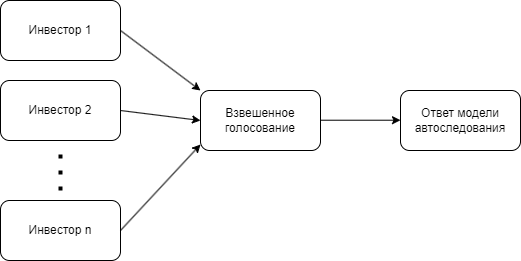
\includegraphics[width=0.8\textwidth]{results/voting.png}}
\caption{Модель автоследования}
\end{figure}

Полученный временной ряд передается в тестируемую модель в качестве дополнительных данных.

\newpage
\subsection{LSTM}

В качестве тестируемой модели используется архитектура Кодировщика - Декодировщика на основе рекуррентной сети LSTM.

\begin{figure}[H]
    \centering
    \begin{minipage}{0.5\textwidth}
        \centering
        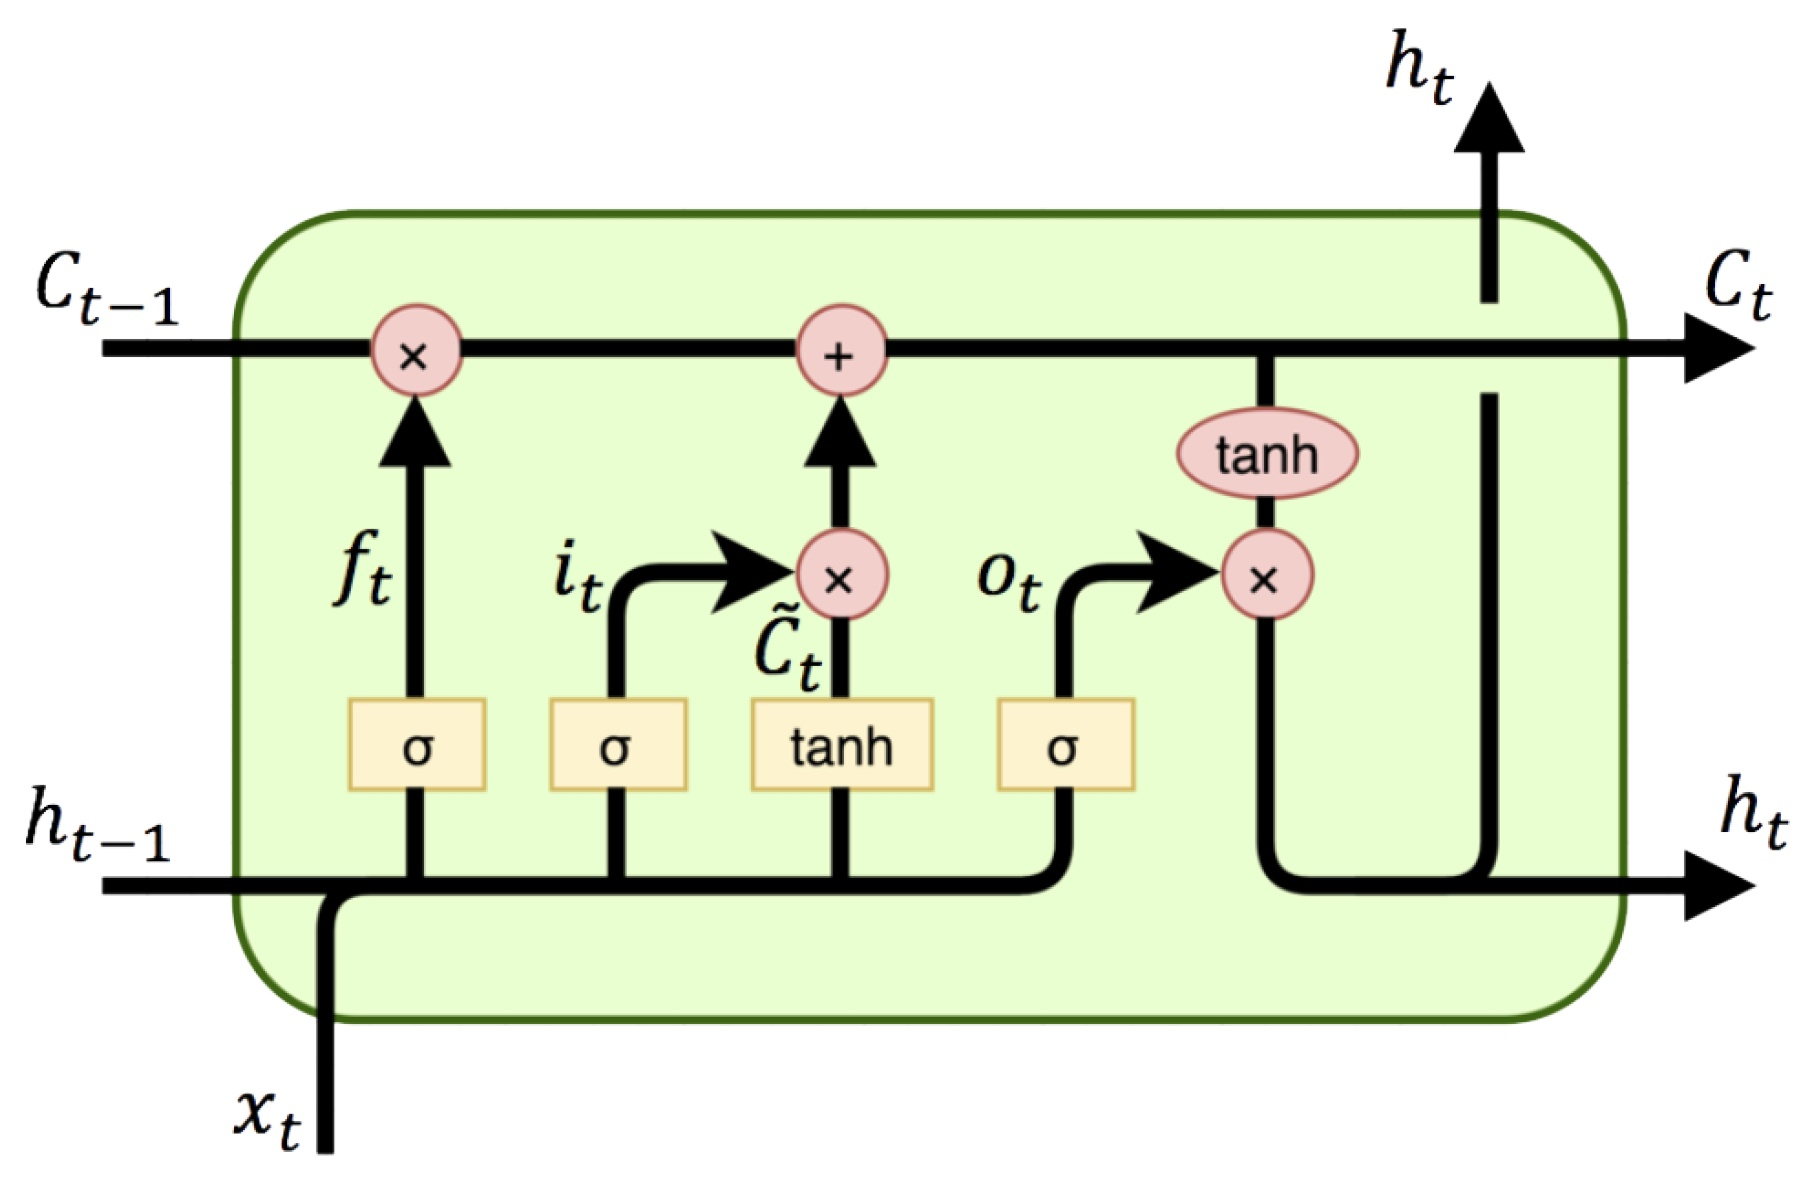
\includegraphics[width=\textwidth]{results/lstm_cell.jpg}
        \caption{Ячейка LSTM~\cite{LSTM3}}
        \label{lstm_cell}
    \end{minipage}
    \hfill
    \begin{minipage}{0.4\textwidth}  
        \begin{align*}
        f_{t} = \sigma (W_{f} [h_{t-1}, x_{t}] +b_{f}) \\
        i_{t} = \sigma (W_{i} [h_{t-1}, x_{t}] + b_{i}) \\
        \widetilde{C_{t}} = \th(W_{C} [h_{t-1}, x_{t}] + b_{C}) \\
        C_{t} = f_{t} \odot C_{t-1} + i_{t} \odot \widetilde{C_{t}} \\
        o_{t} = \sigma (W_{o} [h_{t-1}, x_{t}] + b_{o}) \\
        h_{t} = o_{t} \odot \th(C_{t})
        \end{align*}
    \end{minipage}
\end{figure}

Кодировщик, состоящий из последовательных ячеек LSTM, обрабатывает входную последовательность временного ряда и передает Декодировщику внутреннее представление с последнего шага, которое содержит информацию о всей входной последовательности. Декодировщик, также состоящий из последовательных ячеек LSTM, получает на вход последнее внутрнее представление Кодировщика и использует свои собственные предсказания для генерации последующих значений выходной последовательности.

\begin{figure}[H]\center
{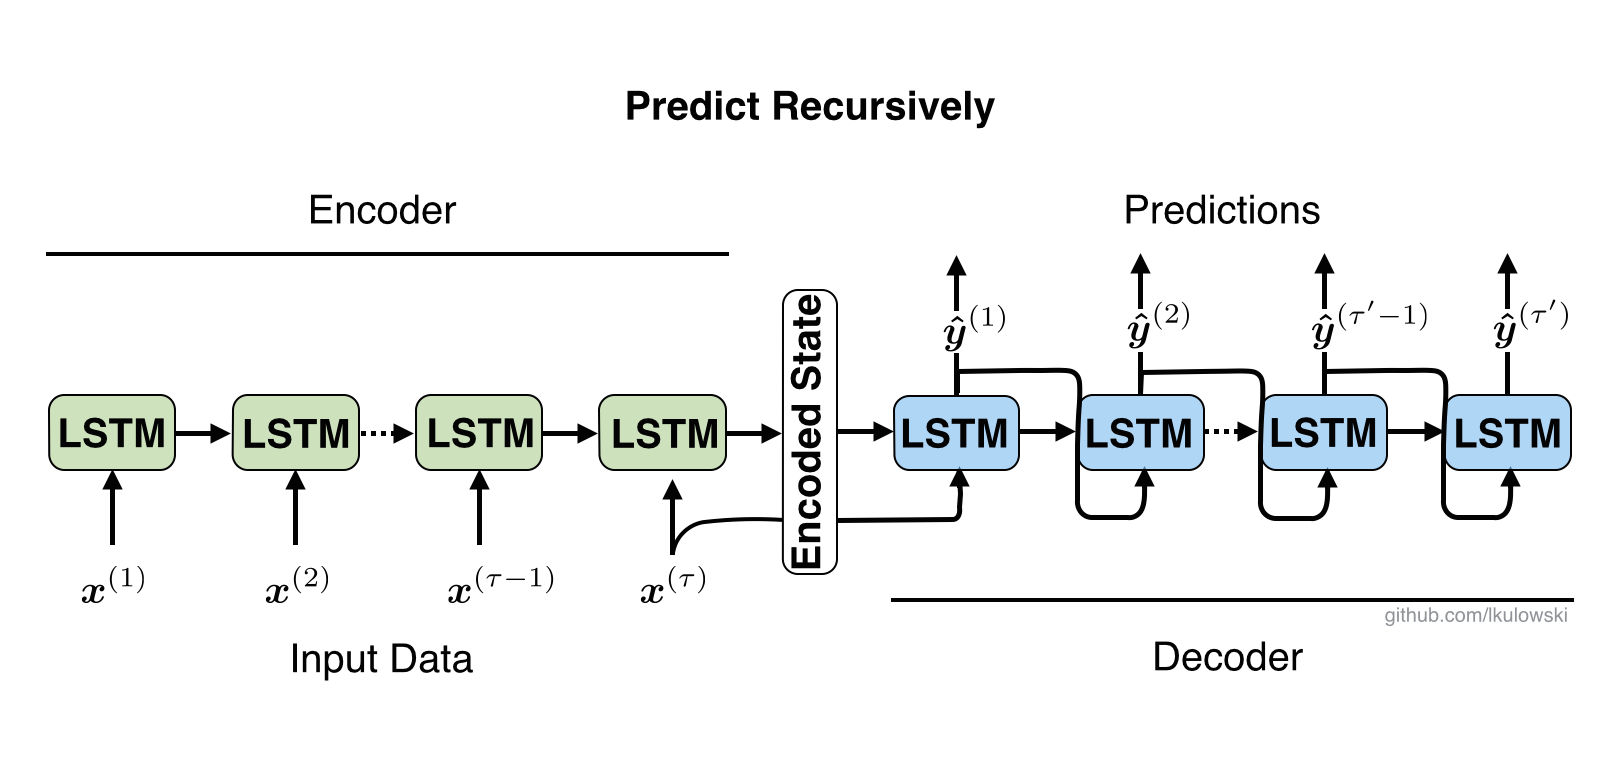
\includegraphics[width=0.8\textwidth]{results/recursive.png}}
\caption{Кодировщик - Декодировщик архитектура на основе LSTM}
\end{figure}


\newpage

Проводится сравнение тестируемой модели с моделями, где в качестве дополнительных данных используются: \\
1) Ответы модели автоследования \\ 
2) Нормальный шум $ \mathcal{N}(0, 1) $

\begin{figure}[H]\center
\subfloat[]
{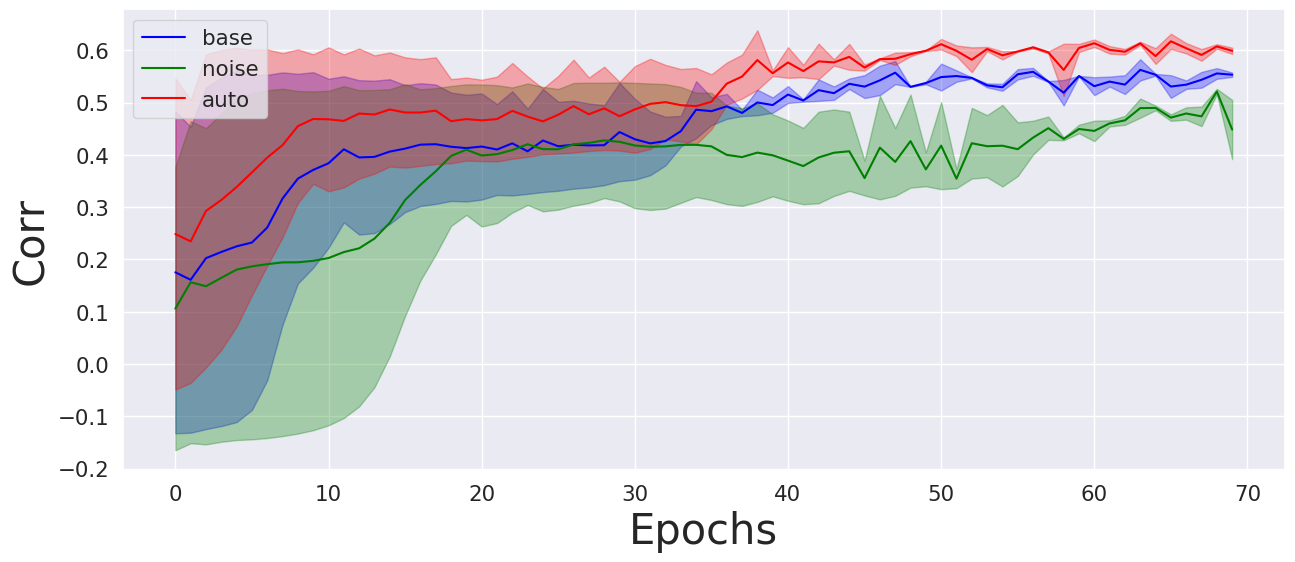
\includegraphics[width=0.5\textwidth]{results/corr_lstm.png}}
\subfloat[]
{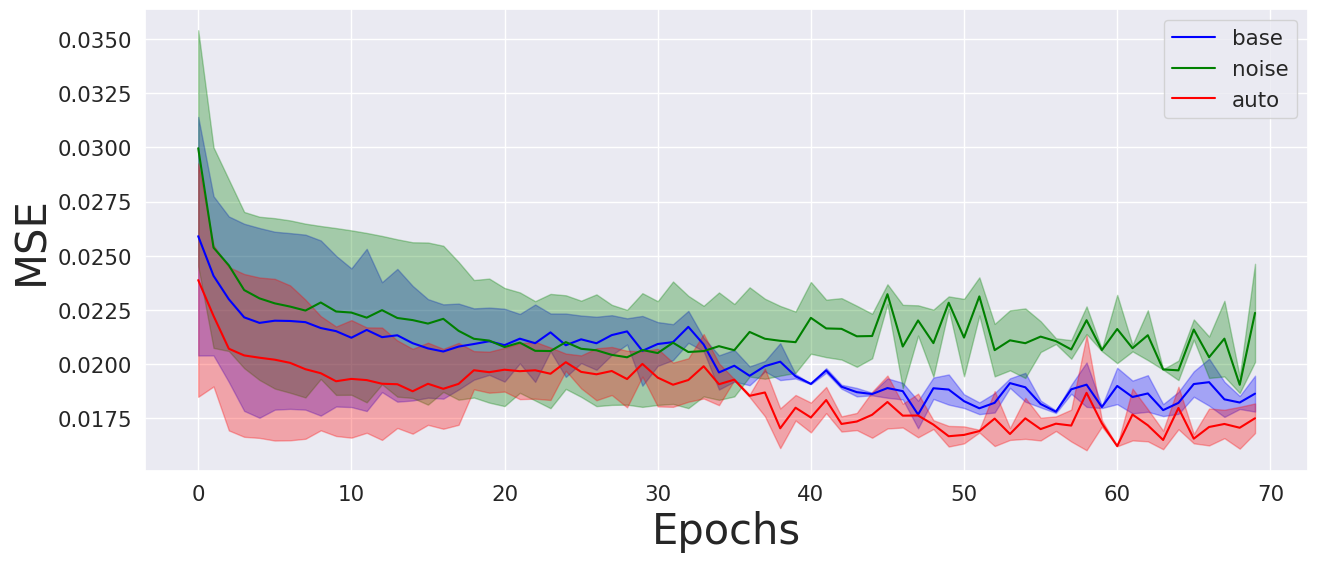
\includegraphics[width=0.5\textwidth]{results/mse_lstm.png}}\\
\caption{Качество аппроксимации на тестовой выборке. Все результаты усреднены по 3 запускам. a) Корреляция Пирсона; b) Средняя квадратичная ошибка}
\label{lstm_plots}
\end{figure}

На рис.~\ref{lstm_plots} показаны графики зависимости корреляции Пирсона и средней квадратичной ошибки на отложенной тестовой выборке между истинными значениями ряда и ответами модели.

На графиках видно, что модель, использующая ответы модели автоследования, показывает лучшее качество прогнозирования, при этом наблюдается снижение средней квадратичной ошибки. 

\begin{table}[H]
\begin{center}
\caption{Качество моделей}
\label{lstm_quality}
\resizebox{\linewidth}{!}{
\begin{tabular}{|c|c|c|c|c|}
\hline
\textbf{Выборка} & \textbf{Модель} & \textbf{\begin{tabular}[c]{@{}c@{}}Дополнительные\\ данные\end{tabular}} & \textbf{\begin{tabular}[c]{@{}c@{}}Корреляция\\ Пирсона\end{tabular}} & \textbf{MSE} \\
\hline
\hline
\multirow{2}{*}{YNDX-Train5} & \multicolumn{1}{|c|}{\multirow{2}{*}{Seq2Seq LSTM}} & --- & $0{,}476 \pm 0{,}027$ & $0{,}0175 \pm 0{,}0003$ \\ \cline{3-3} \cline{4-4} \cline{5-5}
                            & \multicolumn{1}{|c|}{}                                    & Автоследование & $0{,}510 \pm 0{,}036$ & $0{,}0171 \pm 0{,}0001$ \\ 
\hline
\hline
\multirow{2}{*}{YNDX-Train15} & \multicolumn{1}{|c|}{\multirow{2}{*}{Seq2Seq LSTM}} & --- & $0{,}553 \pm 0{,}004$ & $0{,}0186 \pm 0{,}0008$ \\ \cline{3-3} \cline{4-4} \cline{5-5}
                            & \multicolumn{1}{|c|}{}                                    & Автоследование & $0{,}599 \pm 0{,}006$ & $0{,}0175 \pm 0{,}0007$ \\ 
\hline
\hline
\multirow{2}{*}{YNDX-Train30} & \multicolumn{1}{|c|}{\multirow{2}{*}{Seq2Seq LSTM}} & --- & $0{,}478 \pm 0{,}006$ & $0{,}0195 \pm 0{,}0005$ \\ \cline{3-3} \cline{4-4} \cline{5-5}
                            & \multicolumn{1}{|c|}{}                                    & Автоследование & $0{,}538 \pm 0{,}007$ & $0{,}0186 \pm 0{,}0017$ \\ 
\hline
\end{tabular}
}
\end{center}
\end{table}

\newpage 

\begin{figure}[H]\center
{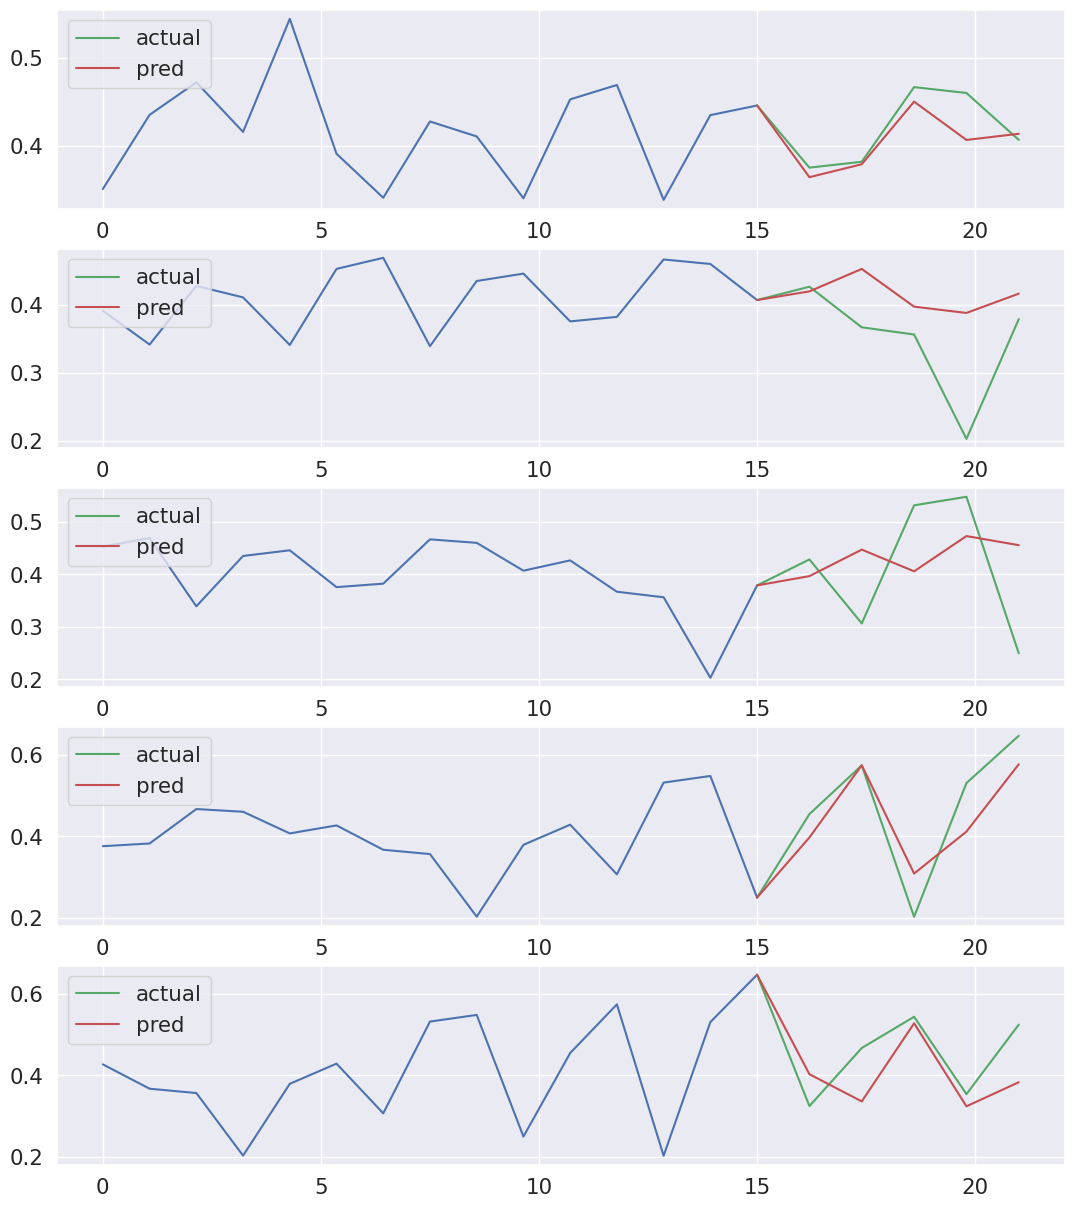
\includegraphics[width=1.0\textwidth]{results/example_lstm.png}}
\caption{Прогнозы LSTM}
\label{example_lstm}
\end{figure}

На рис.~\ref{example_lstm} показаны примеры прогнозов модели Seq2Seq LSTM на отложенной тестовой выборке.

\newpage

\begin{comment}
\subsection{Выбор размера окна}

Нахождение оптимального размера входного окна является одним из основных аспектов в задаче прогнозирования временных рядов. Необходимо найти баланс между захватом достаточной информации и исключением нерелевантных данных. Проведем эксперимент для размера окна равного 5, 15 и 30 в задаче прогнозирования на 5 шагов вперед:

\begin{figure}[H]\center
\subfloat[]
{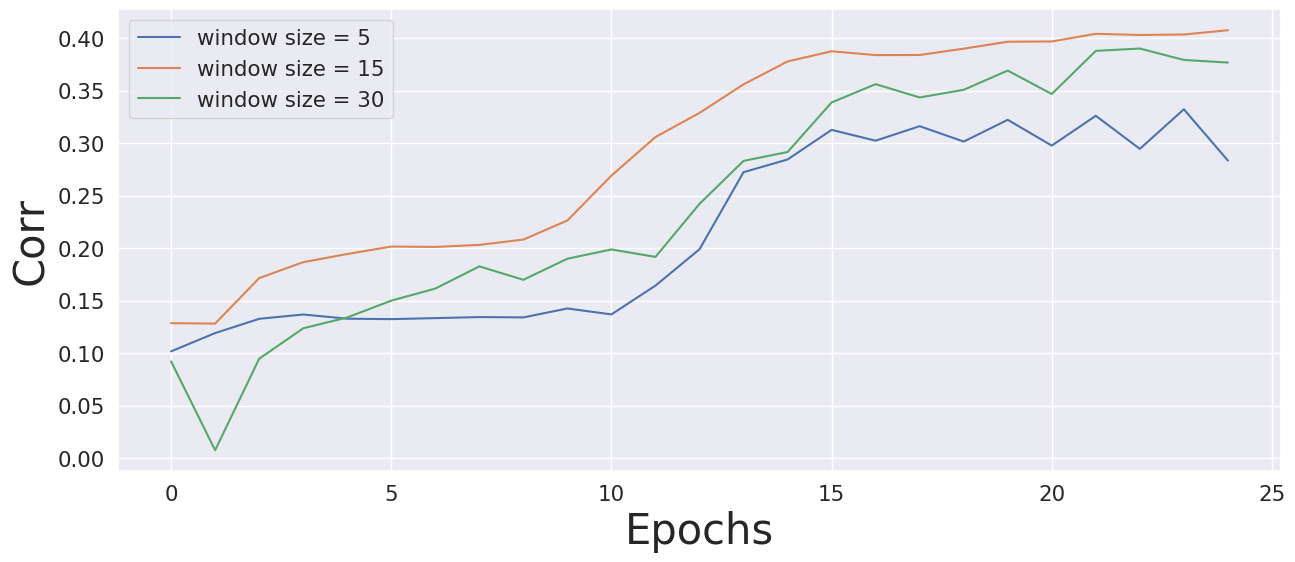
\includegraphics[width=0.5\textwidth]{results/corr_iw.png}}
\subfloat[]
{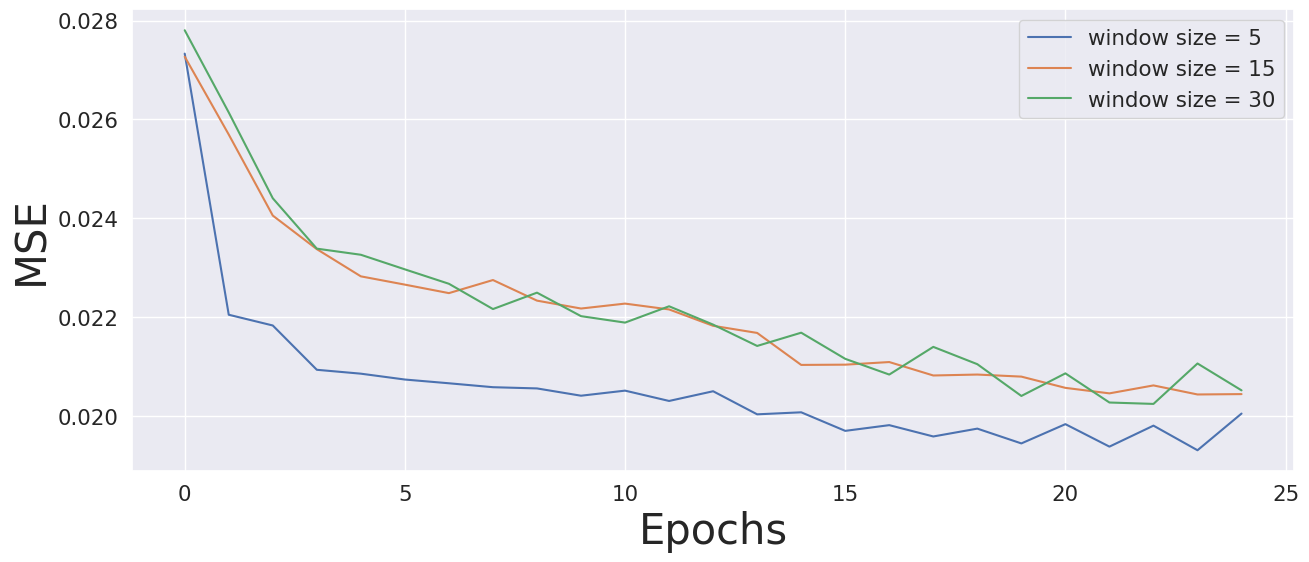
\includegraphics[width=0.5\textwidth]{results/mse_iw.png}}\\
\caption{Корреляция Пирсона и среднеквадратичная ошибка}
\end{figure}

На графиках показаны метрики корреляции Пирсона и среднеквадратичной ошибки в зависимости от горизонта прогнозирования.

Видно, что при размере окна, равного 5 достигается наименьшее значение среднеквадратичной ошибки, однако наибольшее значение корреляции Пирсона достигается при размере окна, равного 15. Для интерпретации метрик посмотрим на визуализацию прогнозов моделей:

\begin{figure}[H]\center
\subfloat[]
{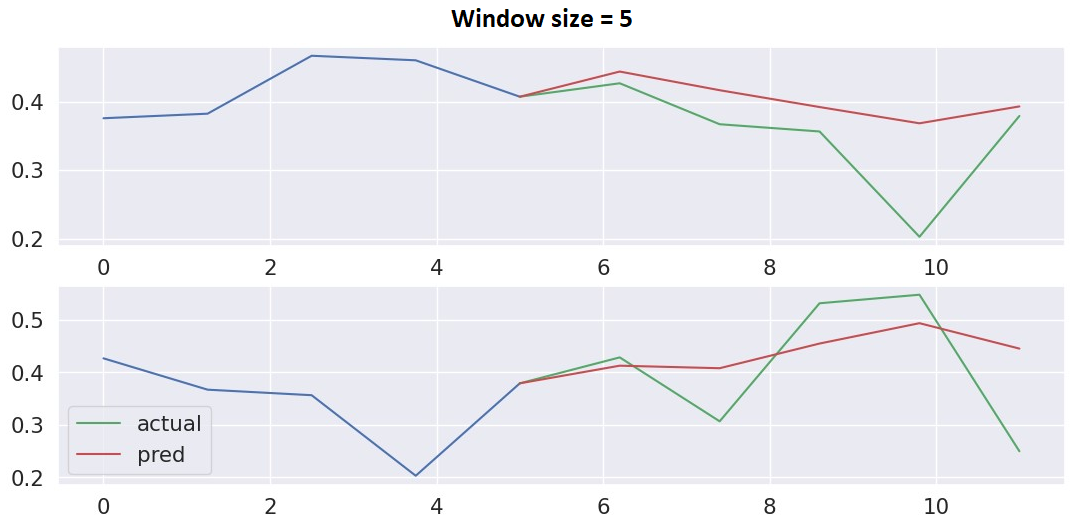
\includegraphics[width=0.5\textwidth]{results/example_iw5.png}}
\subfloat[]
{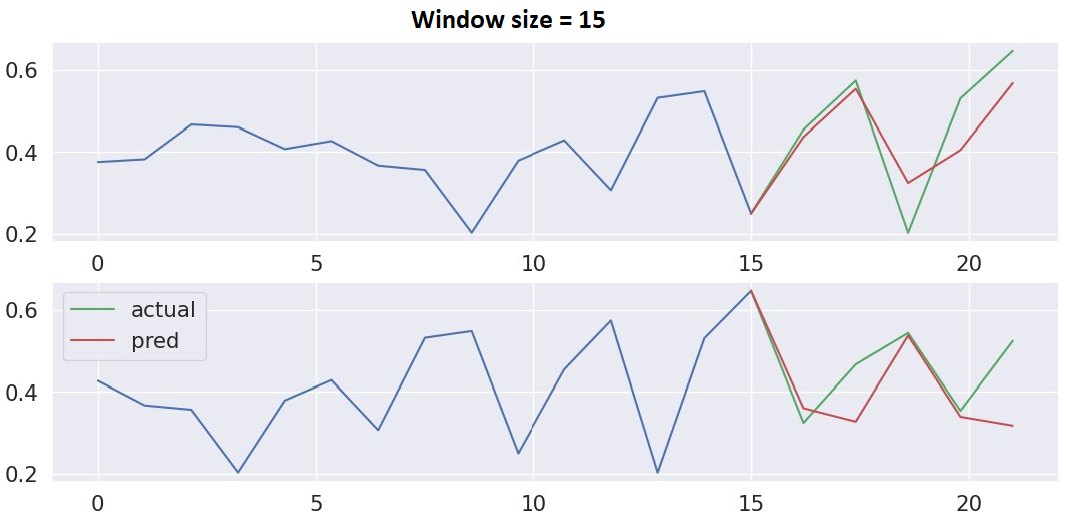
\includegraphics[width=0.5\textwidth]{results/example_iw15.png}}\\
\caption{Прогнозы моделей в зависимости от размера окна}
\end{figure}

Модель, использующая размер входного окна, равного 5, выдает более примитивные паттерны прогноза, что и приводит к меньшему значению среднеквадратичной ошибки. В качестве оптимального выберем размер окна, равный 15.

\end{comment}


\subsection{Горизонт прогнозирования}

Выбор горизонта прогнозирования является одним из основных аспектов в задаче прогнозирования временных рядов. Поскольку используется рекурсивный метод построения прогнозов, то с каждым шагом накапливается ошибка прогноза. Поэтому правильный выбор горизонта позволяет сбалансировать качество прогноза и его пользу для принятия решений. \\

Проводится сравнение модели Seq2Seq LSTM в зависимости от выбранного горизонта прогнозирования.

\begin{figure}[H]\center
\subfloat[]
{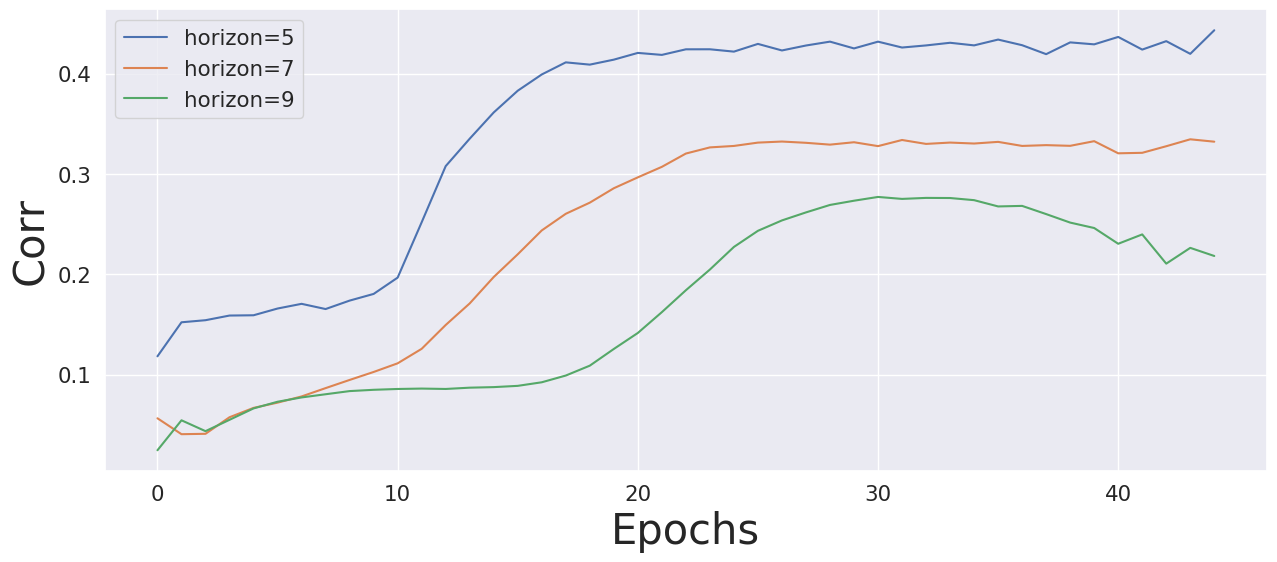
\includegraphics[width=0.5\textwidth]{results/corr_horizon.png}}
\subfloat[]
{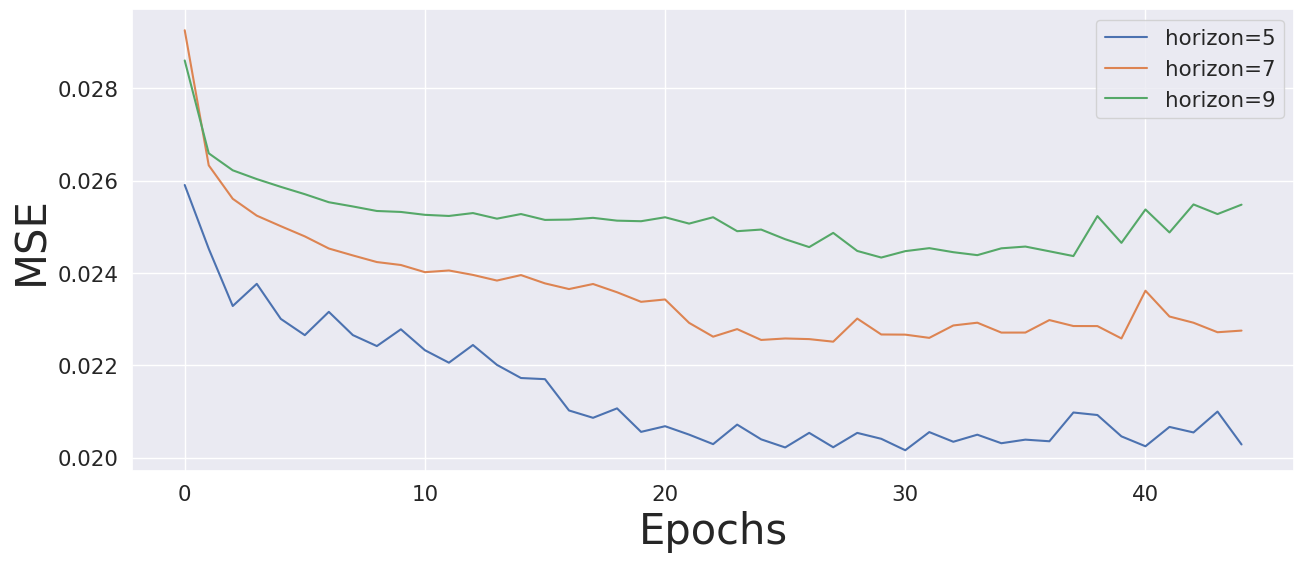
\includegraphics[width=0.5\textwidth]{results/mse_horizon.png}}\\
\caption{Качество аппроксимации на тестовой выборке. a) Корреляция Пирсона; b) Средняя квадратичная ошибка}
\label{horizon_plots}
\end{figure}

На рис.~\ref{horizon_plots} показаны графики зависимости корреляции Пирсона и средней квадратичной ошибки на отложенной тестовой выборке между истинными значениями ряда и ответами модели.

На графиках видно, что с увеличением горизонта прогнозирования качество модели ухудшается. Также наблюдается более поздний выход корреляции Пирсона на плато.

\newpage

\subsection{Transformer}

В качестве тестируемой модели используется архитектура Кодировщика - Декодировщика на основе модели трансформера~\cite{Attention is all you need}.

\begin{figure}[H]
    \begin{minipage}{0.65\textwidth}  
        \begin{enumerate}
            \item Добавляются позиционные векторы $p_{i}$: \\
                $h_{i} = x_{i} + p_{i}, \ H = (h_{1}, ..., h_{n})$
            \item Многомерное самовнимание: \\
                $h_{i}^{j} = \text{Attn}(W_{q}^{j}h_{i}, W_{k}^{j}H, W_{v}^{j}H)$
            \item Конкатенация: \\
                $h_{i}^{'} = \text{MH}_{j}(h_{i}^{j}) \equiv [h_{i}^{1}, ..., h_{i}^{J}]$
            \item Сквозная связь + нормировка уровня: \\
                $h_{i}^{''} = \text{LN}(h_{i}^{'}+h_{i}; \mu_{1}, \sigma_{1})$
            \item Полносвязная 2х-слойная сеть FFN: \\
                $h_{i}^{'''} = W_{2}\text{ReLU}(W_{1}h_{i}^{''}+b_{1}) + b_{2}$
            \item Сквозная связь + нормировка уровня: \\
                $z_{i} = \text{LN}(h_{i}^{'''}+h_{i}^{''}; \mu_{2}, \sigma_{2})$
        \end{enumerate}
    \end{minipage}
    \centering
    \begin{minipage}{0.3\textwidth}
        \centering
        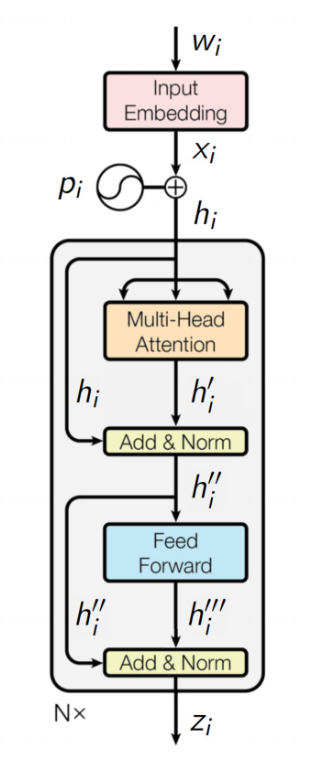
\includegraphics[width=\textwidth]{results/transformer_encoder.png}
        \caption{Трансформер - Кодировщик}
    \end{minipage}
\end{figure}

Трансформер - Кодировщик обрабатывает входную последовательность и передает свои выходы Трансформеру - Декодировщику.

\newpage 

\begin{figure}[H]
    \begin{minipage}{0.7\textwidth}  
        Для всех $t = 1, 2, ...:$
        \begin{enumerate}
            \item Маскирование данных: \\
            $h_{t} = y_{t-1} + p_{t}; \ H_{t} = (h_{1}, ..., h_{t})$
            \item Многомерное самовнимание: \\
            $h_{t}^{'} = \text{LN} \circ \text{MH}_{j} \circ \text{Attn}(W_{q}^{j}h_{t}, W_{k}^{j}H_{t}, W_{v}^{j}H_{t})$
            \item Многомерное внимание на кодировку Z: \\
            $h_{t}^{''} = \text{LN} \circ \text{MH}_{j} \circ \text{Attn}(\tilde{W}_{q}^{j}h_{t}^{'}, \tilde{W}_{k}^{j}Z, \tilde{W}_{v}^{j}Z)$
            \item Двухслойная полносвязная сеть: \\
            $y_{t} = \text{LN} \circ \text{FFN}(h_{t}^{''})$
            \item Линейный предсказывающий слой: \\
            $p(\tilde{w}|t) = \text{SoftMax}_{\tilde{w}}(W_{y}y_{t} + b_{y})$
        \end{enumerate}
        Генерация $\tilde{w}_{t}$
    \end{minipage}
    \centering
    \begin{minipage}{0.25\textwidth}
        \centering
        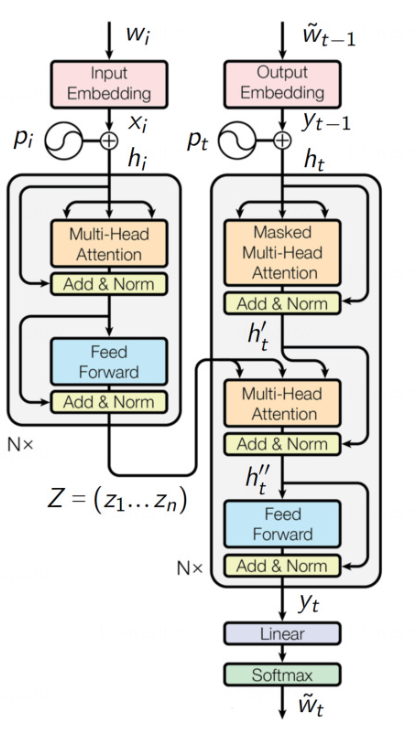
\includegraphics[width=\textwidth]{results/transformer_decoder.png}
        \caption{Трансформер - Декодировщик}
    \end{minipage}
\end{figure}

Трансформер - Декодировщик использует информацию от Трансформера - Кодировщика и генерирует выходную последовательность.

\newpage

Проводится сравнение тестируемой модели с моделью, где в качестве дополнительных данных используются ответы модели автоследования.

\begin{figure}[H]\center
\subfloat[]
{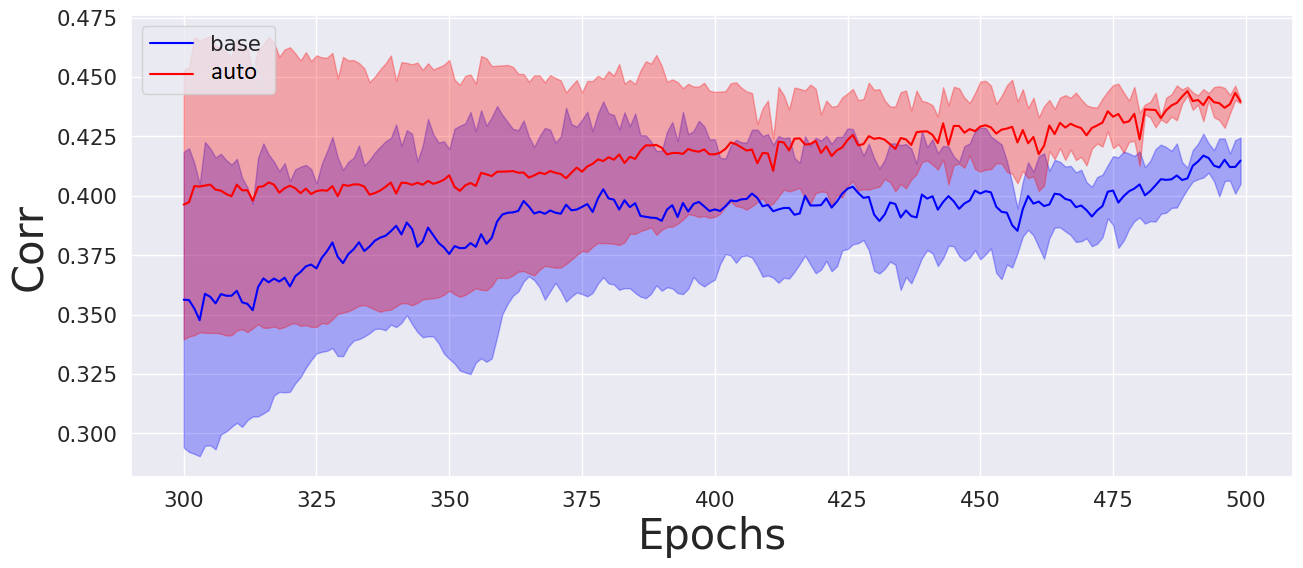
\includegraphics[width=0.5\textwidth]{results/corr_transformer.png}}
\subfloat[]
{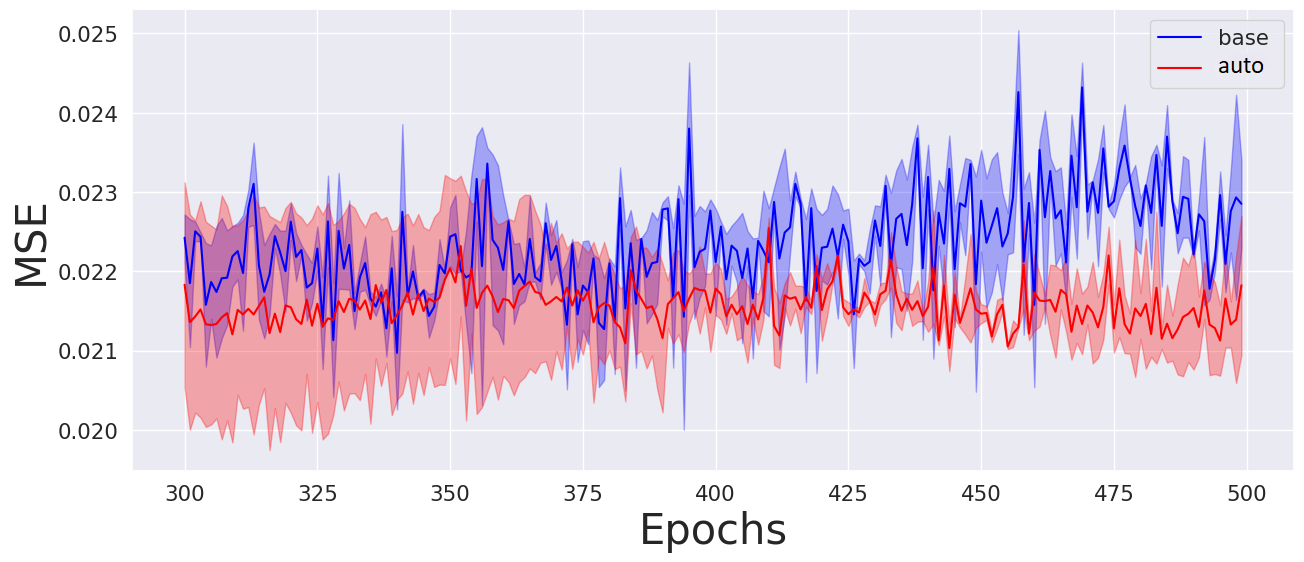
\includegraphics[width=0.5\textwidth]{results/mse_transformer.png}}\\
\caption{Качество аппроксимации на тестовой выборке. Все результаты усреднены по 3 запускам. a) Корреляция Пирсона; b) Средняя квадратичная ошибка}
\label{transformer_plots}
\end{figure}

На рис.~\ref{transformer_plots} показаны графики зависимости корреляции Пирсона и средней квадратичной ошибки на отложенной тестовой выборке между истинными значениями ряда и ответами модели.

На графиках видно, что модель, использующая ответы модели автоследования, показывает лучшее качество прогнозирования, при этом наблюдается снижение средней квадратичной ошибки. 

\begin{table}[H]
\begin{center}
\caption{Качество моделей}
\label{transformer_quality}
\resizebox{\linewidth}{!}{
\begin{tabular}{|c|c|c|c|c|}
\hline
\textbf{Выборка} & \textbf{Модель} & \textbf{\begin{tabular}[c]{@{}c@{}}Дополнительные\\ данные\end{tabular}} & \textbf{\begin{tabular}[c]{@{}c@{}}Корреляция\\ Пирсона\end{tabular}} & \textbf{MSE} \\
\hline
\hline
\multirow{2}{*}{YNDX-Train5} & \multicolumn{1}{|c|}{\multirow{2}{*}{Seq2Seq Transformer}} & --- & $0{,}379 \pm 0{,}039$ & $0{,}0225 \pm 0{,}0005$ \\ \cline{3-3} \cline{4-4} \cline{5-5}
                            & \multicolumn{1}{|c|}{}                                    & Автоследование & $0{,}401 \pm 0{,}035$ & $0{,}0219 \pm 0{,}0004$ \\ 
\hline
\hline
\multirow{2}{*}{YNDX-Train15} & \multicolumn{1}{|c|}{\multirow{2}{*}{Seq2Seq Transformer}} & --- & $0{,}415 \pm 0{,}010$ & $0{,}0229 \pm 0{,}0006$ \\ \cline{3-3} \cline{4-4} \cline{5-5}
                            & \multicolumn{1}{|c|}{}                                    & Автоследование & $0{,}440 \pm 0{,}001$ & $0{,}0218 \pm 0{,}0009$ \\ 
\hline
\hline
\multirow{2}{*}{YNDX-Train30} & \multicolumn{1}{|c|}{\multirow{2}{*}{Seq2Seq Transformer}} & --- & $0{,}406 \pm 0{,}011$ & $0{,}0211 \pm 0{,}0010$ \\ \cline{3-3} \cline{4-4} \cline{5-5}
                            & \multicolumn{1}{|c|}{}                                    & Автоследование & $0{,}425 \pm 0{,}009$ & $0{,}0210 \pm 0{,}0009$ \\ 
\hline
\end{tabular}
}
\end{center}
\end{table}

\newpage

\begin{figure}[H]\center
{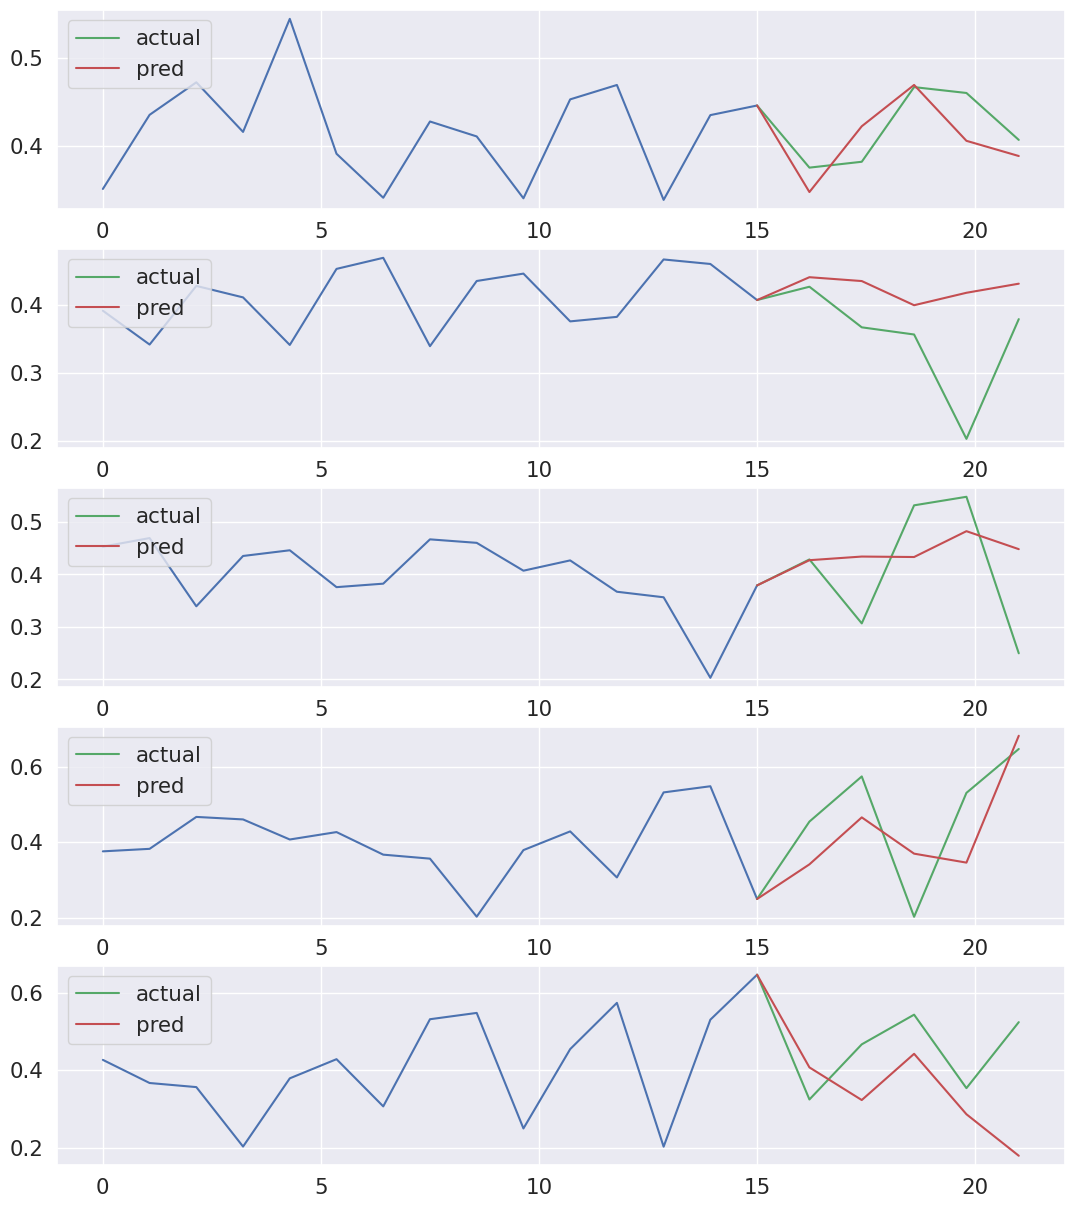
\includegraphics[width=1.0\textwidth]{results/example_transformer.png}}
\caption{Прогнозы Transformer}
\label{example_transformer}
\end{figure}

На рис.~\ref{example_transformer} показаны примеры прогнозов модели Seq2Seq Transformer на отложенной тестовой выборке.

\newpage

\subsection{Код вычислительного эксперимента}

Весь код вычислительного эксперимента представлен в~\cite{Github}. Также доступны письменный отчет и результаты экспериментов.